\documentclass[10pt, letterpaper]{article}

\usepackage[margin=1in]{geometry}
\usepackage[utf8]{inputenc}
\usepackage[T1]{fontenc}
\usepackage{lmodern}
\usepackage{amsmath, amssymb, amsthm}
\usepackage{booktabs}
\usepackage{graphicx}
\usepackage{xcolor}
\usepackage{hyperref}
\usepackage{enumitem}
\usepackage{caption, subcaption}
\usepackage{listings}
\usepackage{tikz}
\usetikzlibrary{positioning, fit, calc, arrows.meta}

% Theorem environments
\newtheorem{theorem}{Theorem}[section]
\newtheorem{lemma}[theorem]{Lemma}
\newtheorem{proposition}[theorem]{Proposition}
\newtheorem{corollary}[theorem]{Corollary}
\theoremstyle{definition}
\newtheorem{definition}[theorem]{Definition}
\newtheorem{example}[theorem]{Example}
\theoremstyle{remark}
\newtheorem{remark}[theorem]{Remark}

% Lean code formatting
\lstdefinelanguage{Lean}{
  morekeywords={def, theorem, lemma, axiom, variable, inductive, structure,
    class, instance, where, match, with, by, exact, intro, apply, simp,
    rfl, fun, let, have, show, calc, if, then, else, do, return, sorry,
    namespace, end, open, import, section, Type, Prop, True, False,
    forall, exists, private, set, obtain, push_neg, unfold, constructor,
    rintro, refine, subst, rw, cases, induction, congr, ext},
  sensitive=true,
  morecomment=[l]{--},
  morecomment=[n]{/-}{-/},
  morestring=[b]",
  literate={→}{$\to$}1 {←}{$\leftarrow$}1 {↔}{$\leftrightarrow$}1
           {∀}{$\forall$}1 {∃}{$\exists$}1 {¬}{$\lnot$}1
           {∧}{$\land$}1 {∨}{$\lor$}1 {⟨}{$\langle$}1 {⟩}{$\rangle$}1
           {₁}{$_1$}1 {₂}{$_2$}1 {₀}{$_0$}1
           {⊊}{$\subsetneq$}1
           {≠}{$\neq$}1,
}
\lstset{
  language=Lean,
  basicstyle=\ttfamily\small,
  keywordstyle=\bfseries\color{blue!70!black},
  commentstyle=\itshape\color{green!50!black},
  stringstyle=\color{red!60!black},
  breaklines=true,
  columns=flexible,
  frame=single,
  framesep=4pt,
  xleftmargin=8pt,
  xrightmargin=8pt,
  aboveskip=8pt,
  belowskip=8pt,
}

% Notation
\newcommand{\Sach}{\mathsf{S}}
\newcommand{\World}{\mathsf{World}}
\newcommand{\Prop}{\mathsf{Prop}}
\newcommand{\eval}{\mathsf{eval}}
\newcommand{\expresses}{\mathsf{expresses}}
\newcommand{\structEq}{\sim_{\mathrm{struct}}}
\newcommand{\formEq}{\sim_{\mathrm{form}}}
\newcommand{\semEq}{\sim_{\mathrm{sem}}}
\newcommand{\Lean}{\textsc{Lean}}

\title{What \Lean{} Cannot Say:\\
A Machine-Checked Analysis of Wittgenstein's \emph{Tractatus}}
\author{Robb Walters}
\date{April 2026}

\begin{document}
\maketitle

\begin{abstract}
We present a machine-checked reconstruction of the semantic core
of \emph{Tractatus Logico-Philosophicus} in the \Lean{} proof
assistant.  The formalization models objects, states of affairs,
worlds, and propositions, and proves truth-functional
compositionality, functional completeness, and bivalence.

Beyond encoding, the system is parameterized over world models,
allowing a precise separation between (i)~structural invariants
of the propositional syntax, (ii)~model-dependent assumptions
such as the independence of atomic facts, and (iii)~formal limits
of expressibility.  We show that truth-functional compositionality
holds in all models, while independence characterizes a specific
``free'' model and fails in constrained models.

To analyze the relation between object language and metalanguage,
we introduce an \texttt{expresses} relation linking propositions
to meta-level predicates.  Using this, we prove that any
proposition expressing a world-independent property must be a
tautology or contradiction.  Consequently, nontrivial propositions
cannot express world-independent truths.

We further distinguish three notions of
equivalence---syntactic identity, logical-form equivalence up to
permutation, and semantic equivalence---and prove their strict
separation.

These results yield a formal decomposition of the \emph{Tractatus}
into invariants, assumptions, and limits, and provide a precise
characterization of the saying/showing distinction as a theorem
about expressibility in truth-functional languages.
The formalization comprises 1,517 lines of \Lean~4, proves 50
theorem and lemma declarations with 0 \texttt{sorry} obligations
and 1 deliberate axiom (\texttt{axiom silence : True}, encoding
TLP~7).%
\footnote{The formalization is publicly available at
  \url{https://leangenius.org/proof/tractatus-ontology}.
  It builds with \Lean~4 (toolchain \texttt{leanprover/lean4:v4.17.0}),
  depends on Mathlib (\texttt{import Mathlib.Tactic}), and compiles via
  \texttt{lake build}.  See Appendix~\ref{app:build} for full
  instructions.}
\end{abstract}

% ================================================================
\section{Introduction}
\label{sec:intro}
% ================================================================

Wittgenstein's \emph{Tractatus Logico-Philosophicus}~\cite{wittgenstein1921}
proposes that the world consists of atomic facts (Sachverhalte),
that propositions are truth-functions of elementary propositions,
and that the limits of language are the limits of the world.
The text is terse, aphoristic, and deliberately resistant to
formalization---yet its semantic core is a precise theory of
truth-functional composition that invites formal reconstruction.

Several authors have pursued this invitation.
Lokhorst~\cite{lokhorst1988} provides a set-theoretic
reconstruction covering ontology, semantics, and propositional
attitudes;
Fogelin~\cite{fogelin1987} initiates the debate over expressive
completeness that Geach~\cite{geach1981} and
Soames~\cite{soames1983} develop;
Miller~\cite{miller1995} develops a Tractarian semantics for
predicate logic, responding in part to Fogelin and
Carruthers~\cite{carruthers1989};
Weiss~\cite{weiss2017} reconstructs the logical system with
$\Pi^1_1$-completeness results;
Stokhof~\cite{stokhof2008} traces the \emph{Tractatus}'s
influence on formal semantics.
These reconstructions clarify the \emph{Tractatus} as a semantic
system but are carried out on paper, without machine verification.
Separately, the proof-assistant community has formalized
philosophical arguments~\cite{benzmuller2017,fitelson2007} and
even complete metaphysical systems~\cite{scherf2025}, but a
Tractarian formalization has not appeared.

This paper contributes a machine-checked reconstruction in
\Lean~4~\cite{moura2021} that goes beyond encoding to yield new
analytical results.  Our central claim is:

\begin{quote}
\emph{The saying/showing distinction of the \emph{Tractatus} can
be reformulated as a theorem: nontrivial propositions cannot
express world-independent truths.}
\end{quote}

\noindent
This is not a paraphrase of Wittgenstein but a provable
consequence of the typed structure of the formalization.
The key device is an \texttt{expresses} relation (Definition~\ref{def:expresses})
that bridges the object language (propositions of type
$\mathsf{Proposition}\;\Sach$) and the metalanguage (terms of
type $\Prop$), making the object/meta boundary visible at the
type level.

More broadly, by parameterizing the formalization over a general
\texttt{WorldModel} structure, we show that the claims of the
\emph{Tractatus} decompose into three classes:
\begin{enumerate}[nosep]
  \item \textbf{Structural invariants} that hold in every world
    model---compositionality, bivalence, De Morgan duality.
  \item \textbf{Model-dependent assumptions} that hold in the
    unconstrained ``free'' model but fail in constrained
    models---principally, the independence of atomic facts.
  \item \textbf{Formal limits} on expressibility---the collapse
    of world-independent content to tautology or contradiction,
    and the strict separation of syntactic, logical-form, and
    semantic equivalence.
\end{enumerate}

\noindent
The specific contributions of this paper are:
\begin{enumerate}[nosep, label=(\arabic*)]
  \item A parameterized world-model abstraction that cleanly
    separates structural invariants from modeling assumptions,
    enabling precise identification of which Tractarian claims
    are theorems of the syntax and which are properties of a
    particular world model (Section~\ref{sec:formalization}).
  \item An \texttt{expresses} relation that makes the object/meta
    boundary a typed distinction, yielding the expressibility
    collapse theorem (Theorem~\ref{thm:collapse}): any proposition
    expressing a world-independent property is a tautology or
    contradiction (Section~\ref{sec:limits}).
  \item An equivalence hierarchy $\structEq \subsetneq \formEq
    \subsetneq \semEq$ with strict separation witnesses, providing
    a formal candidate for Wittgenstein's ``logical form''
    (Section~\ref{sec:hierarchy}).
  \item A three-way decomposition of all 50 formalized results
    into invariants, assumptions, and limits
    (Table~\ref{tab:decomposition}, Appendix~\ref{app:theorems}).
  \item A first-order extension using higher-order abstract syntax,
    proving compositionality lifts to quantified propositions
    (Section~\ref{sec:firstorder}).
\end{enumerate}

\noindent
The formalization comprises 1,517 lines of \Lean~4 across two
files.\footnote{%
  \texttt{TractatusOntology.lean} (1,229 lines, 41 theorem/lemma
  declarations) and \texttt{TractatusQuantifiers.lean} (288 lines,
  9 theorem declarations), plus 1 deliberate axiom.
  Appendix~\ref{app:theorems} lists every declaration.}
All proofs compile with 0 \texttt{sorry} obligations.
The sole axiom is \texttt{axiom silence : True} (TLP~7), a
deliberate boundary marker discussed in
Section~\ref{sec:limitations}.

The paper is organized as follows.
Section~\ref{sec:formalization} presents the formalization:
types, evaluation, and the world-model abstraction.
Section~\ref{sec:invariants} establishes the structural
invariants.
Section~\ref{sec:assumptions} analyzes the model-dependent
assumptions and exhibits countermodels.
Section~\ref{sec:limits} proves the expressibility results and
the equivalence hierarchy.
Section~\ref{sec:related} discusses related work.
Section~\ref{sec:discussion} reflects on the philosophical
implications and limitations.

% ================================================================
\section{The Formalization}
\label{sec:formalization}
% ================================================================

We formalize the ontological skeleton of the \emph{Tractatus}
in \Lean~4.  The design choices are deliberate modeling
decisions, not exegetical claims about Wittgenstein's intent.
We state them explicitly so that the reader can assess the
reconstruction's scope and limitations.

\begin{remark}[Choice of proof assistant]
\label{rem:lean4}
We use \Lean~4~\cite{moura2021} rather than Coq, Isabelle, or
Agda for three reasons: (i)~its dependent type theory allows
definitions and proofs to coexist naturally, which suits a
formalization that mixes data definitions with metatheorems;
(ii)~the Mathlib library provides automation
(\texttt{simp}, \texttt{tauto}, \texttt{push\_neg}) that keeps
proofs concise; and (iii)~\Lean's tactic mode allows readable
proof scripts that can be presented in a paper without excessive
notation overhead.
\end{remark}

\begin{remark}[Classical logic]
\label{rem:classical}
The formalization assumes classical logic throughout, via
\texttt{Classical.em} and related principles imported from
Mathlib.  This is a deliberate choice matching the
\emph{Tractatus}'s bivalent semantics: every proposition is
either true or false in every world (TLP~4.023).
Theorems depending essentially on classical reasoning include
bivalence, excluded middle as a tautology, double negation,
the expressibility collapse theorem, and contingent-proposition
variation.  A constructive formalization would require
restricting the world model or weakening several results.
\end{remark}

% ----------------------------------------------------------------
\subsection{Objects and States of Affairs}
\label{sec:objects}
% ----------------------------------------------------------------

TLP~2.02: ``The object is simple.''  Objects are the substance
of the world (TLP~2.021).  We model them as an abstract type
\texttt{TractObject} with no internal structure, capturing
Wittgenstein's insistence on simplicity.

A state of affairs (Sachverhalt) is a possible combination of
objects (TLP~2.01).  Rather than encoding the combinatorial
structure of objects into states of affairs, we index states of
affairs by an abstract type~$\Sach$:

\begin{lstlisting}
variable (TractObject : Type)
variable (Sachverhalt : Type)
\end{lstlisting}

\noindent
This choice leaves the internal structure of states of affairs
unspecified---an interpretive decision that captures independence
while remaining agnostic about combinatorial form (cf.\
TLP~2.0141).

% ----------------------------------------------------------------
\subsection{Worlds}
\label{sec:worlds}
% ----------------------------------------------------------------

TLP~1: ``The world is everything that is the case.''
A world is determined by which states of affairs obtain.  We
model this as a predicate:

\begin{lstlisting}
def World := Sachverhalt → Prop
\end{lstlisting}

\noindent
Every function $\Sach \to \Prop$ counts as a world.  This gives
the full Boolean cube of truth-value assignments, making the
independence of atomic facts (TLP~2.061) hold by construction.
We return to this modeling choice and its consequences in
Section~\ref{sec:assumptions}.

% ----------------------------------------------------------------
\subsection{Propositions}
\label{sec:propositions}
% ----------------------------------------------------------------

TLP~5: ``The proposition is a truth-function of elementary
propositions.''  We define propositions as an inductive type
built from elementary propositions, negation, and conjunction:

\begin{lstlisting}
inductive Proposition (S : Type) where
  | elementary : S → Proposition S
  | neg        : Proposition S → Proposition S
  | conj       : Proposition S → Proposition S → Proposition S
\end{lstlisting}

\noindent
Disjunction, implication, biconditional, and NAND are defined as
derived operations (TLP~5.101, 5.5), confirming that $\{\lnot, \land\}$
is an adequate basis.

% ----------------------------------------------------------------
\subsection{Semantic Evaluation}
\label{sec:eval}
% ----------------------------------------------------------------

The core semantic function interprets propositions against a
world:

\begin{lstlisting}
def Proposition.eval (p : Proposition S) (w : World S) : Prop :=
  match p with
  | .elementary s => w s
  | .neg q        => ¬ (q.eval w)
  | .conj q r     => q.eval w ∧ r.eval w
\end{lstlisting}

\noindent
An elementary proposition $\mathtt{elementary}\;s$ is true in
world~$w$ exactly when $w\;s$ holds.  Negation and conjunction
lift to their classical counterparts.%
\footnote{The formalization also provides a
\texttt{Bool}-valued evaluator \texttt{evalBool} for decidable
computation and proves its correctness against
\texttt{eval} (Theorem \texttt{evalBool\_correct}).
This engineering artifact enables \texttt{\#eval} demonstrations
but is not philosophically load-bearing.}

% ----------------------------------------------------------------
\subsection{Tautology, Contradiction, Nontriviality}
\label{sec:tautology}
% ----------------------------------------------------------------

A proposition is a \emph{tautology} if it holds in every world,
a \emph{contradiction} if it holds in none, and
\emph{nontrivial} if it holds in some world and fails in
another:

\begin{lstlisting}
def IsTautology (p : Proposition S) : Prop :=
  ∀ w : World S, p.eval w
def IsContradiction (p : Proposition S) : Prop :=
  ∀ w : World S, ¬ (p.eval w)
def Nontrivial (p : Proposition S) : Prop :=
  ∃ w₁ w₂ : World S, p.eval w₁ ∧ ¬ p.eval w₂
\end{lstlisting}

\noindent
We prove that nontriviality is equivalent to being neither a
tautology nor a contradiction
(Theorem~\texttt{nontrivial\_iff\_not\_taut\_not\_contra}).

% ----------------------------------------------------------------
\subsection{General World Models}
\label{sec:worldmodel}
% ----------------------------------------------------------------

The definitions above hardwire the world model: every function
$\Sach \to \Prop$ is a world.  In many applications---physics,
epistemic logic, constrained databases---not every assignment is
legitimate.  We introduce a \texttt{WorldModel} structure to
parameterize the semantics:

\begin{lstlisting}
structure WorldModel (S : Type) where
  W        : Type
  holds    : W → S → Prop
  nonempty : Nonempty W
\end{lstlisting}

\noindent
The \emph{free model} \texttt{freeModel} recovers the original
semantics: $W = \Sach \to \Prop$ and \texttt{holds} is function
application.  We define a general evaluator \texttt{evalM} and
prove that \texttt{evalM (freeModel S)} agrees with
\texttt{Proposition.eval} (Theorem~\texttt{evalM\_free\_eq\_eval}).

This abstraction is the key structural device of the
formalization.  It allows us to state precisely which results
depend on the choice of world model and which do not.

% ================================================================
\section{Structural Invariants}
\label{sec:invariants}
% ================================================================

The following results hold in \emph{every} world model---they
are consequences of the inductive structure of propositions and
classical logic alone, with no assumptions about which worlds
exist.

% ----------------------------------------------------------------
\subsection{Truth-Functional Compositionality}
\label{sec:compositionality}
% ----------------------------------------------------------------

\begin{theorem}[Compositionality, model-independent]
\label{thm:compositionality}
For any world model $M$, any proposition $p$, and any two
worlds $w_1, w_2 \in M.W$: if $M.\mathit{holds}\;w_1\;s
\leftrightarrow M.\mathit{holds}\;w_2\;s$ for every state of
affairs~$s$, then $\eval_M\;p\;w_1 \leftrightarrow
\eval_M\;p\;w_2$.
\end{theorem}

\noindent
The proof is by structural induction on propositions.
The elementary case follows from the hypothesis; negation and
conjunction lift via \texttt{Iff.not} and \texttt{Iff.and}.

\begin{lstlisting}
theorem truth_functional_compositionality_gen (p : Proposition S)
    (w₁ w₂ : M.W)
    (h : ∀ s : S, M.holds w₁ s ↔ M.holds w₂ s) :
    evalM M p w₁ ↔ evalM M p w₂ := by
  induction p with
  | elementary s => exact h s
  | neg q ih     => simp only [evalM]; exact ih.not
  | conj q r ihq ihr => simp only [evalM]; exact ihq.and ihr
\end{lstlisting}

\noindent
This establishes TLP~5 as a structural invariant: the
truth-value of a compound proposition is determined by its
elementary constituents regardless of which worlds the model
admits.

% ----------------------------------------------------------------
\subsection{Bivalence and Classical Tautologies}
\label{sec:bivalence}
% ----------------------------------------------------------------

Elementary bivalence (TLP~4.023) is an instance of classical
excluded middle:

\begin{theorem}[Bivalence]
For any state of affairs~$s$ and world~$w$: $w\;s \lor \lnot\;w\;s$.
\end{theorem}

\noindent
The standard tautologies follow: excluded middle ($p \lor
\lnot p$), double negation ($\lnot\lnot p \leftrightarrow p$),
De Morgan's laws, and modus ponens.  We verify each as a formal
theorem.  All of these results depend on \texttt{Classical.em}
(see Remark~\ref{rem:classical}).

% ----------------------------------------------------------------
\subsection{NAND Functional Completeness}
\label{sec:nand}
% ----------------------------------------------------------------

TLP~5.5 anticipates the Sheffer stroke.  We prove that negation
and conjunction are both expressible via NAND:

\begin{theorem}[NAND completeness]
\label{thm:nand}
For any propositions $p$, $q$ and world $w$:
\begin{enumerate}[nosep]
  \item $\mathtt{nand}(p, p).\eval\;w \leftrightarrow
    (\lnot p).\eval\;w$
  \item $(\lnot\;\mathtt{nand}(p, q)).\eval\;w \leftrightarrow
    (p \land q).\eval\;w$
\end{enumerate}
\end{theorem}

\noindent
Since $\{\lnot, \land\}$ generates all truth-functions and NAND
generates $\{\lnot, \land\}$, NAND alone is functionally
complete over the set of truth-functions expressible by the
proposition type---confirming TLP~5.5.

% ================================================================
\section{Model-Dependent Assumptions}
\label{sec:assumptions}
% ================================================================

Not every claim in the \emph{Tractatus} is a structural
invariant.  The independence of atomic facts---perhaps the most
famous ontological thesis of the text---is a property of a
specific world model.

% ----------------------------------------------------------------
\subsection{Independence in the Free Model}
\label{sec:independence}
% ----------------------------------------------------------------

We formalize independence as a typeclass:

\begin{lstlisting}
class IndependentWorlds (S : Type) where
  realizable : ∀ assignment : S → Prop,
    ∃ w : World S, ∀ s, w s ↔ assignment s
\end{lstlisting}

\noindent
The free model trivially satisfies this: every assignment
\emph{is} a world.

\begin{lstlisting}
instance : IndependentWorlds S :=
  ⟨fun a => ⟨a, fun _ => Iff.rfl⟩⟩
\end{lstlisting}

\noindent
Independence is thus not a theorem about logic but a consequence
of the modeling choice $\World\;\Sach = \Sach \to \Prop$.
This distinction---between what is proved and what is assumed by
the encoding---is precisely the kind of clarification that a
typed formalization forces.

% ----------------------------------------------------------------
\subsection{Failure in Constrained Models}
\label{sec:constrained}
% ----------------------------------------------------------------

To show that independence is genuinely contingent on the model,
we exhibit two countermodels.

\paragraph{Abstract countermodel.}
Consider two states of affairs $a, b$ with $a \neq b$, where
$b$ must co-occur with $a$.  Define
$\mathtt{ConstrainedWorld}\;\Sach\;a\;b = \{w : \Sach \to \Prop
\mid w\;a \to w\;b\}$.  Then:

\begin{theorem}[Independence fails in constrained models]
\label{thm:constrained}
If $a \neq b$, then there is no constrained world realizing the
assignment $\{a \mapsto \top, b \mapsto \bot\}$.
\end{theorem}

\begin{lstlisting}
theorem constrained_independence_fails (a b : S) (hab : a ≠ b) :
    ¬ ∀ assignment : S → Prop,
      ∃ cw : ConstrainedWorld S a b,
        ∀ s, cw.val s ↔ assignment s := by
  intro h
  let bad : S → Prop := fun s => s = a
  obtain ⟨⟨w, hw⟩, hmatch⟩ := h bad
  have ha : w a := (hmatch a).mpr rfl
  have hb : w b := hw ha
  exact hab ((hmatch b).mp hb)
\end{lstlisting}

\paragraph{Weather model.}
A more concrete example: three states of affairs (rain, clouds,
snow) with the physical constraint \emph{rain implies clouds}.
The weather model restricts worlds to those satisfying this
constraint.

\begin{theorem}[Weather model]
\label{thm:weather}
In the weather model, there is no world where rain holds but
clouds does not.
\end{theorem}

\noindent
These results make explicit a point that is often asserted
informally: TLP~2.061 (``Atomic facts are independent of one
another'') is not a logical law but a constraint on the space of
possible worlds.  Our formalization turns this observation into a
proof.

Notably, Wittgenstein himself later retreated from the
independence thesis.  In ``Some Remarks on Logical
Form''~\cite{wittgenstein1929}, he acknowledged that the
color-exclusion problem---the mutual incompatibility of
determinate color predicates (e.g., a point cannot be both red
and blue)---demonstrates that certain atomic facts are not
logically independent.  Our constrained models formalize
precisely this kind of failure: the weather model's constraint
that rain implies clouds is structurally analogous to the
color-exclusion problem.  In both cases, physical or conceptual
constraints on states of affairs reduce the space of possible
worlds below the full Boolean cube.

% ================================================================
\section{Formal Limits: Expressibility and Equivalence}
\label{sec:limits}
% ================================================================

The deepest results of the formalization concern the boundaries
of what the object language can express.  These are not claims
within the Tractarian system but \emph{about} it---theorems at
the meta-level that formalize Wittgenstein's saying/showing
distinction.

% ----------------------------------------------------------------
\subsection{The \texttt{expresses} Relation}
\label{sec:expresses}
% ----------------------------------------------------------------

We introduce a typed bridge between the object language and the
metalanguage:

\begin{definition}[\texttt{expresses}]
\label{def:expresses}
A proposition $p : \mathsf{Proposition}\;\Sach$ \emph{expresses}
a meta-level property $P : \Prop$ if and only if $p$'s truth
value tracks $P$ in every world:
\[
  \expresses\;p\;P \;\;\stackrel{\mathrm{def}}{=}\;\;
  \forall\;w : \World\;\Sach,\;\; p.\eval\;w \leftrightarrow P
\]
\end{definition}

\begin{lstlisting}
def expresses (p : Proposition S) (P : Prop) : Prop :=
  ∀ w : World S, p.eval w ↔ P
\end{lstlisting}

\noindent
The type signature makes the object/meta distinction visible:
$p$ lives in the object language, $P$ lives in \Lean's
metalanguage, and \texttt{expresses} is the claim that they
correspond.  This is the formalization's key analytical device.

% ----------------------------------------------------------------
\subsection{Expressibility Collapse}
\label{sec:collapse}
% ----------------------------------------------------------------

\begin{theorem}[Expressibility collapse]
\label{thm:collapse}
If a proposition $p$ expresses a world-independent property
$P : \Prop$, then $p$ is a tautology or a contradiction.
\end{theorem}

\begin{proof}
Suppose $\expresses\;p\;P$ holds.  Then for any two worlds
$w_1, w_2$:
\[
  p.\eval\;w_1 \;\leftrightarrow\; P \;\leftrightarrow\;
  p.\eval\;w_2
\]
so $p$ has the same truth value in all worlds.  By excluded
middle on $p.\eval\;w_0$ for an arbitrary world~$w_0$, either
$p$ holds everywhere (tautology) or fails everywhere
(contradiction).
\end{proof}

\begin{lstlisting}
theorem saying_showing_triviality (q : Proposition S)
    (P : Prop) [Nonempty S]
    (h : expresses q P) :
    IsTautology q ∨ IsContradiction q := by
  apply world_constant_taut_or_contra
  intro w₁ w₂
  exact (h w₁).trans (h w₂).symm
\end{lstlisting}

\noindent
The contrapositive is immediate and philosophically sharper:

\begin{corollary}[Nontrivial propositions cannot express
world-independent content]
\label{cor:nontrivial}
If $p$ is nontrivial (i.e., true in some world and false in
another), then there is no $P : \Prop$ such that
$\expresses\;p\;P$.
\end{corollary}

\begin{lstlisting}
theorem nontrivial_cannot_express_world_independent
    (p : Proposition S) (P : Prop) [Nonempty S]
    (hnt : Nontrivial p) :
    ¬ expresses p P := by
  intro h
  exact nontrivial_expressibility_requires_world_dependence
    p P hnt h
\end{lstlisting}

\noindent
This is the paper's headline result.  It says: if a proposition
genuinely ``says'' something---i.e., carves out a nontrivial
region of logical space---then what it says cannot be a
world-independent truth.  Genuine content requires variation
across possible worlds.  What is world-independent can only be
``shown'' by the structure of the formalism itself, not ``said''
within it.

This transforms the saying/showing distinction from a
philosophical thesis into a provable constraint on
truth-functional languages.

\begin{remark}[On the definitional character of the collapse]
\label{rem:triviality}
A natural objection is that the expressibility collapse theorem
is \emph{trivial}: since $P : \Prop$ is world-independent by
construction (it is a closed term in \Lean's metalanguage), the
collapse to tautology or contradiction follows almost
definitionally from the definition of \texttt{expresses}.

We acknowledge this.  The proof is indeed short---two lines of
tactic code.  The contribution lies not in the proof's
difficulty but in three aspects of the \emph{formulation}:

\emph{(a) Making the object/meta boundary typed.}  The
definition of \texttt{expresses} forces the distinction between
$p : \mathsf{Proposition}\;\Sach$ (object language) and
$P : \Prop$ (metalanguage) to be a type-level constraint.  This
makes the boundary machine-checkable rather than merely
conventional.

\emph{(b) The analogy to other definitional results in logic.}
Many foundational results in logic are ``definitional'' in
a similar sense.  Tarski's undefinability theorem rests on the
diagonal lemma, which is itself a consequence of how truth
predicates are defined.  The incompleteness theorems depend on
the coding of syntax.  In each case, the contribution is the
\emph{conceptual apparatus} that makes the result statable, not
the complexity of the derivation.  Our \texttt{expresses}
relation plays an analogous role: it provides the vocabulary in
which the saying/showing distinction becomes a theorem.

\emph{(c) The constraint is genuinely informative.}
The collapse theorem rules out a precise class of claims:
no nontrivial proposition can serve as a ``name'' for a fixed
metalinguistic truth.  This is not obvious from the definition
of \texttt{expresses} alone---one must also establish
(via \texttt{world\_constant\_taut\_or\_contra}) that
world-invariant truth values force triviality.
\end{remark}

\begin{remark}[The \texttt{Nonempty S} assumption]
\label{rem:nonempty}
Several key theorems---including the expressibility collapse
(Theorem~\ref{thm:collapse}), \texttt{world\_constant\_taut\_or\_contra},
and \texttt{structEq\_ne\_semEq}---require \texttt{[Nonempty S]},
i.e., that the type of states of affairs is inhabited.

This assumption is philosophically motivated: a world with no
possible states of affairs is degenerate in the Tractarian
framework.  TLP~1 (``The world is everything that is the case'')
presupposes that there are things that could be the case.
When $\Sach$ is empty, the only world is the trivial
predicate, every proposition is a tautology, and the
interesting structure collapses.  The assumption
\texttt{[Nonempty S]} excludes this degenerate case.

Technically, the assumption is used to construct a witness
world in which to evaluate propositions.  For the collapse
theorem, we need at least one world to case-split on; for the
equivalence hierarchy, we need at least one atom to
construct separating witnesses.
\end{remark}

% ----------------------------------------------------------------
\subsection{The Equivalence Hierarchy}
\label{sec:hierarchy}
% ----------------------------------------------------------------

The formalization distinguishes three notions of proposition
equivalence, ordered by strictness:

\begin{definition}[Equivalence hierarchy]
\label{def:hierarchy}
Let $p, q : \mathsf{Proposition}\;\Sach$.
\begin{enumerate}[nosep]
  \item \textbf{Structural equivalence} ($p \structEq q$):
    $p$ and $q$ are built from identical constructors in the
    same tree shape with identical atoms.
  \item \textbf{Logical-form equivalence} ($p \formEq q$):
    there exists a bijective renaming of atoms (a permutation
    $\sigma : \Sach \xrightarrow{\sim} \Sach$) such that
    $p.\mathtt{rename}\;\sigma = q$.
  \item \textbf{Semantic equivalence} ($p \semEq q$):
    $p$ and $q$ have the same truth value in every world:
    $\forall w,\; p.\eval\;w \leftrightarrow q.\eval\;w$.
\end{enumerate}
\end{definition}

\noindent
We prove that $\formEq$ is an equivalence relation (reflexive by
the identity permutation, symmetric by inverse, transitive by
composition) and establish the strict hierarchy:

\begin{theorem}[Strict separation]
\label{thm:hierarchy}
$\structEq \;\subsetneq\; \formEq \;\subsetneq\; \semEq$
\end{theorem}

\begin{proof}
Each inclusion is witnessed by containment and a separating example.

\emph{$\structEq \subsetneq \formEq$:}
Structural equality implies propositional equality (by induction),
which implies logical-form equivalence via the identity
permutation.  Strictness: $\mathtt{elementary}(\mathit{rain})$
and $\mathtt{elementary}(\mathit{snow})$ are $\formEq$ (via the
swap permutation) but not $\structEq$ (different atoms).

\emph{$\formEq \subsetneq \semEq$:}
Logical-form equivalence implies truth-table isomorphism
(Theorem~\texttt{formEq\_implies\_truth\_table\_iso}): there
exists a world-relabeling $f$ such that $p.\eval\;w
\leftrightarrow q.\eval\;(f\;w)$ for all $w$.
When this relabeling is the identity, semantic equivalence
follows.  However, $\formEq$ does \emph{not} imply $\semEq$ in
general---the relabeling need not be trivial.
Strictness: $\lnot\lnot(\mathtt{elementary}\;s)$
is $\semEq$ to $\mathtt{elementary}\;s$ (by double negation) but
not $\formEq$ (renaming preserves tree depth, so a depth-3 tree
cannot become depth-1).
\end{proof}

% --- Equivalence Hierarchy Figure ---
\begin{figure}[t]
\centering
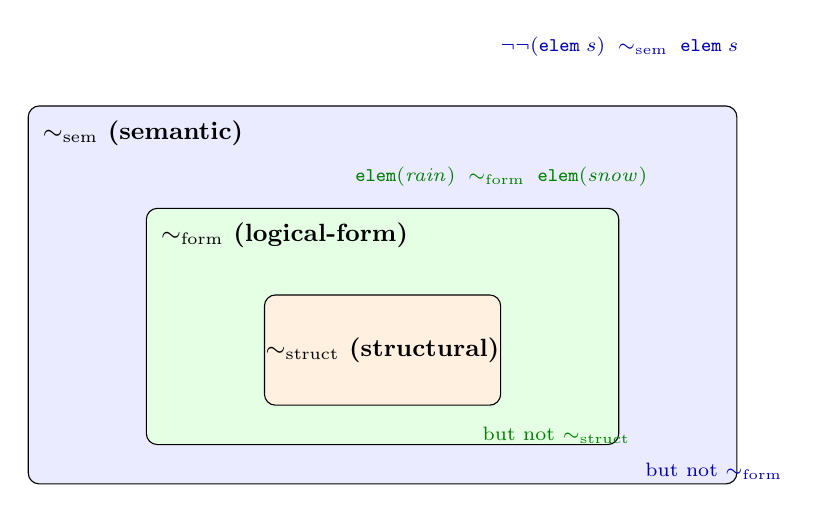
\begin{tikzpicture}[
  node distance=0.8cm,
  every node/.style={font=\small},
  box/.style={draw, rounded corners, minimum width=3.2cm,
              minimum height=0.7cm, align=center},
]
  % Nested containment boxes (drawn as rounded rectangles)
  \node[box, fill=blue!8, minimum width=9.0cm, minimum height=4.8cm]
    (sem) {};
  \node[box, fill=green!10, minimum width=6.0cm, minimum height=3.0cm]
    at ([yshift=-0.4cm]sem.center) (form) {};
  \node[box, fill=orange!12, minimum width=3.0cm, minimum height=1.4cm]
    at ([yshift=-0.3cm]form.center) (struct) {};

  % Labels
  \node[anchor=north west, font=\small\bfseries] at ([xshift=2pt, yshift=-2pt]sem.north west)
    {$\semEq$ (semantic)};
  \node[anchor=north west, font=\small\bfseries] at ([xshift=2pt, yshift=-2pt]form.north west)
    {$\formEq$ (logical-form)};
  \node[font=\small\bfseries] at (struct.center)
    {$\structEq$ (structural)};

  % Witnesses for strict separation
  \node[font=\scriptsize, text=blue!70!black, anchor=south]
    at ([yshift=0.5cm]sem.north west -| form.east)
    {$\lnot\lnot(\mathtt{elem}\;s) \;\semEq\; \mathtt{elem}\;s$};
  \node[font=\scriptsize, text=blue!70!black, anchor=north]
    at ([yshift=-0.1cm, xshift=1.2cm]form.south east)
    {but not $\formEq$};

  \node[font=\scriptsize, text=green!50!black, anchor=south]
    at ([yshift=0.15cm, xshift=0cm]form.north west -| struct.east)
    {$\mathtt{elem}(\mathit{rain}) \;\formEq\; \mathtt{elem}(\mathit{snow})$};
  \node[font=\scriptsize, text=green!50!black, anchor=north]
    at ([yshift=-0.15cm, xshift=0.7cm]struct.south east)
    {but not $\structEq$};
\end{tikzpicture}
\caption{The equivalence hierarchy with strict separation
  witnesses.  Each inclusion is proper: $\structEq \subsetneq
  \formEq \subsetneq \semEq$.}
\label{fig:hierarchy}
\end{figure}

\noindent
Figure~\ref{fig:hierarchy} illustrates the hierarchy.  This
clarifies a long-standing ambiguity in the
\emph{Tractatus}.  Wittgenstein's notion of ``logical form''
(TLP~4.0141) is neither syntactic identity nor truth-conditional
equivalence but something in between.  Our $\formEq$---defined
via bijective atom renaming---provides a formal candidate:
it captures the connective structure while abstracting over
which particular atoms appear.  The strict separation proves
that this intermediate notion is genuine, not collapsible into
either extreme.

% ----------------------------------------------------------------
\subsection{First-Order Extension}
\label{sec:firstorder}
% ----------------------------------------------------------------

In a companion file (\texttt{TractatusQuantifiers.lean}), we
extend the propositional calculus with first-order quantifiers
using higher-order abstract syntax (HOAS):

\begin{lstlisting}
inductive FOProp (S : Type) (D : Type) : Type where
  | lift     : Proposition S → FOProp S D
  | negFO    : FOProp S D → FOProp S D
  | conjFO   : FOProp S D → FOProp S D → FOProp S D
  | forall_  : (D → FOProp S D) → FOProp S D
  | exists_  : (D → FOProp S D) → FOProp S D
\end{lstlisting}

\noindent
The HOAS encoding leverages \Lean's metalanguage for variable
binding, avoiding explicit substitution machinery.  This
substantially reduces proof overhead but ties the formalization
more tightly to \Lean's metatheory than a de Bruijn index
encoding would---in particular, induction over HOAS terms
requires care, since the recursor for HOAS inductives must track
the functional argument.

We prove that compositionality lifts to the first-order level:

\begin{theorem}[First-order compositionality]
\label{thm:fo-comp}
For any $p : \mathsf{FOProp}\;\Sach\;D$ and worlds $w_1, w_2$
agreeing on all states of affairs, $p.\eval\;w_1 \leftrightarrow
p.\eval\;w_2$.
\end{theorem}

\noindent
We also establish eight additional results: universal--existential
duality (TLP~5.52), universal distribution over conjunction,
existential distribution over disjunction (reverse direction),
lift preservation, vacuous quantifier elimination (requiring
\texttt{Nonempty D}), double negation at the first-order level,
De Morgan duality for quantifiers, and first-order bivalence.

This section is preliminary.  The results proved are standard
consequences of the semantic definitions.  The philosophically
interesting question---whether Wittgenstein's $N$-operator can
ground quantification over infinite domains---requires a
separate formalization of the $N$-operator, which is deferred to
future work.  The file notes the
Geach--Soames critique~\cite{geach1981,soames1983}: for infinite
domains, Wittgenstein's claim that quantifiers reduce to
applications of the $N$-operator is problematic, since the
$N$-operator is a finitary syntactic operation.  For finite
domains the connection is unproblematic and will be established
when the $N$-operator formalization is available.

% ================================================================
\section{Related Work}
\label{sec:related}
% ================================================================

\paragraph{Formal reconstructions of the \emph{Tractatus}.}
Lokhorst~\cite{lokhorst1988} provides the most comprehensive
prior formal reconstruction, covering ontology, semantics, and
propositional attitudes in a set-theoretic framework.  His
axiomatization of independence and his truth-functionality
theorem (every sentence is a truth-function of elementary
sentences) overlap with our encoding, but he does not formalize
the saying/showing boundary itself.
Weiss~\cite{weiss2017} gives a 50-page reconstruction of the
\emph{Tractatus}'s logical system, analyzing the $N$-operator
and form-series in detail and proving that tautology-hood is
$\Pi^1_1$-complete for countable domains---a striking
complexity result that sharpens the Geach--Soames critique.
Miller~\cite{miller1995} develops a Tractarian semantics for
predicate logic that is independent of the metaphysics of
logical atomism, engaging with both Fogelin's~\cite{fogelin1987}
critique of expressive completeness and Carruthers'~\cite{carruthers1989}
book-length treatment of Tractarian semantics.
Stokhof~\cite{stokhof2008} reads the \emph{Tractatus} as a
proto-formal semantics, tracing its influence through Carnap's
state descriptions to possible-worlds semantics, and argues
that the saying/showing distinction arises from the
universalism of the framework---a philosophical diagnosis our
expressibility collapse theorem makes precise.
All of these works provide formal clarity but are carried out
on paper; none offers machine-checked proofs, and none
parameterizes over world models to isolate which claims are
structural invariants versus modeling assumptions.

\paragraph{The expressive completeness debate.}
Fogelin~\cite{fogelin1987} initiates the modern debate over
whether the \emph{Tractatus}'s logical resources are
expressively complete.  Geach~\cite{geach1981} argues that the
$N$-operator cannot ground quantification over infinite domains,
since it is a finitary operation.
Soames~\cite{soames1983} sharpens this: the \emph{Tractatus}'s
claim that all of logic reduces to truth-functional operations
on elementary propositions is undermined when the domain of
quantification is infinite.
Carruthers~\cite{carruthers1989} provides a sympathetic
reconstruction of Tractarian semantics that attempts to address
some of these concerns.
Our formalization takes the critique seriously: the first-order
extension (Section~\ref{sec:firstorder}) uses standard
quantifiers rather than the $N$-operator, and notes the
finite-domain connection as a separate theorem to be proved only
when an $N$-operator formalization is available.

\paragraph{Proof assistants and philosophy.}
Benzm\"uller and colleagues~\cite{benzmuller2017} have used
Isabelle to formalize ontological arguments and modal logic.
Their approach uses shallow semantic embeddings of higher-order
modal logic into Isabelle's metalogic, which contrasts with our
direct encoding in dependent type theory: we define the
Tractarian object language explicitly as an inductive type,
whereas shallow embeddings reuse the proof assistant's logic
as the object logic.
Fitelson and Zalta~\cite{fitelson2007} pioneer ``computational
metaphysics,'' using automated reasoners to verify theorems
in abstract-object theory.
Scherf~\cite{scherf2025} provides the most directly comparable
work: a machine-checked axiomatization of Advaita Ved\=anta in
\Lean~4 (69 axioms, 40+ theorems), demonstrating that complete
philosophical systems can be formalized in dependent type
theory.
Corfield~\cite{corfield2020} argues at book length that
homotopy type theory is a better logic for philosophy than
predicate logic, but provides no machine-checked formalizations.
To our knowledge, no prior work formalizes any part of the
\emph{Tractatus} in any proof assistant, nor uses the type
system to isolate the saying/showing boundary as a provable
constraint.

% ================================================================
\section{Discussion}
\label{sec:discussion}
% ================================================================

% ----------------------------------------------------------------
\subsection{What the Formalization Shows}
\label{sec:shows}
% ----------------------------------------------------------------

The formalization yields three kinds of insight.

First, it makes the \emph{Tractatus}'s implicit modeling
decisions explicit.  The choice $\World\;\Sach = \Sach \to
\Prop$ is not neutral: it builds independence into the
foundations.  By parameterizing over \texttt{WorldModel}, we
separate what follows from the propositional syntax (compositionality)
from what follows from the choice of world space (independence).
This distinction is available in principle but rarely made
precise in the philosophical literature.

Second, it transforms the saying/showing distinction from a
metaphilosophical thesis into a theorem with a two-line proof.
The \texttt{expresses} relation is the key: once the
object/meta boundary is a type distinction, the collapse result
(Theorem~\ref{thm:collapse}) follows by transitivity of
biconditional.  See Remark~\ref{rem:triviality} for a
discussion of the definitional character of this result and
why the formulation is nonetheless a genuine contribution.

Third, the equivalence hierarchy (Theorem~\ref{thm:hierarchy})
provides a precise formal candidate for Wittgenstein's
notion of ``logical form.''  The strict separation $\structEq
\subsetneq \formEq \subsetneq \semEq$ shows that logical form,
understood as connective structure up to atom permutation, is a
genuine intermediate notion that cannot be reduced to either
syntax or semantics.

% ----------------------------------------------------------------
\subsection{Limitations}
\label{sec:limitations}
% ----------------------------------------------------------------

Several aspects of the \emph{Tractatus} lie beyond the scope of
this formalization.

\paragraph{Object structure.}
The type $\Sach$ is abstract: we do not model how objects combine
into states of affairs.  TLP~2.0141 (``The possibility of its
occurrence in atomic facts is the form of the object'') suggests
a richer dependent-type encoding where the form of an object
constrains its combinatorial possibilities.  This would make
independence a substantive theorem rather than a definitional
consequence.

\paragraph{The $N$-operator.}
Wittgenstein's claim that all propositions can be generated from
elementary propositions by successive applications of a single
operation (TLP~6) is not formalized here.  The $N$-operator is
a finitary syntactic construction, and its connection to
quantification over infinite domains remains philosophically
contentious (Section~\ref{sec:firstorder}).

\paragraph{The picture theory.}
The \emph{Tractatus}'s claim that propositions are
\emph{pictures} of reality (TLP~2.1--2.174) involves a notion
of structural isomorphism between language and world that goes
beyond truth-functional evaluation.  Our formalization captures
the truth-conditional aspect but not the pictorial-isomorphism
aspect.

\paragraph{Self-reference and the ladder.}
TLP~6.54 famously declares that the propositions of the
\emph{Tractatus} itself are ``nonsensical'' and must be ``thrown
away'' after use.  Our formalization is, by design, a
metalanguage that talks \emph{about} the Tractarian object
language.  It cannot formalize its own status as a ladder to be
discarded---this is the point where type theory, like any formal
system, reaches its own saying/showing boundary.

We mark this boundary with a deliberate axiom:

\begin{lstlisting}
axiom silence : True
\end{lstlisting}

\noindent
This is not a missing proof but a design boundary.  The axiom
states nothing contentful ($\mathtt{True}$ is already provable);
it marks the point where the formalization acknowledges its own
limits.

\paragraph{Future work.}
Natural extensions include: (i)~formalizing the $N$-operator and
proving the finite-domain quantifier connection;
(ii)~enriching the object structure via dependent types to make
independence substantive; (iii)~investigating the picture theory
as a structural isomorphism between proposition trees and
world-fragments; and (iv)~exploring connections to homotopy type
theory, where the ``same logical form'' relation might be
formalized as a path in a suitable type.

% ================================================================
\section{Conclusion}
\label{sec:conclusion}
% ================================================================

We have presented a machine-checked reconstruction of the
semantic core of \emph{Tractatus Logico-Philosophicus} in
\Lean~4.  The formalization proves 50 theorems and lemmas across
two files, decomposes the
\emph{Tractatus} into structural invariants, model-dependent
assumptions, and formal limits of expressibility, and
characterizes the saying/showing distinction as a theorem:
nontrivial propositions cannot express world-independent truths.

The equivalence hierarchy $\structEq \subsetneq \formEq
\subsetneq \semEq$ provides a typed decomposition of the space
between syntax and semantics, isolating logical form as a
genuine intermediate structure.

These results suggest that proof assistants are a productive tool
for philosophical analysis---not merely for verifying known
results, but for revealing structural constraints that are
invisible when the analysis is conducted on paper.

The formalization is publicly available at
\url{https://leangenius.org/proof/tractatus-ontology}.

% ================================================================
% Appendix
% ================================================================

\appendix

% ----------------------------------------------------------------
\section{Build Instructions}
\label{app:build}
% ----------------------------------------------------------------

The formalization is built with \Lean~4 using the \texttt{lake}
build system.  To reproduce:

\begin{enumerate}[nosep]
  \item Install \Lean~4 via \texttt{elan}:
    \texttt{curl -sSf https://raw.githubusercontent.com/leanprover/elan/master/elan-init.sh | sh}
  \item Clone the repository:
    \texttt{git clone https://github.com/leangenius/tractatus-ontology.git}
  \item The \texttt{lean-toolchain} file pins the version to
    \texttt{leanprover/lean4:v4.17.0}.
  \item The \texttt{lakefile.lean} declares a dependency on Mathlib
    (the formalization uses \texttt{import Mathlib.Tactic}).
  \item Build: \texttt{lake build}
\end{enumerate}

\noindent
The build produces zero errors, zero warnings, and zero
\texttt{sorry} obligations.  The sole axiom
(\texttt{axiom silence : True}) is intentional and
discussed in Section~\ref{sec:limitations}.

Proof files:
\begin{itemize}[nosep]
  \item \texttt{proofs/TractatusOntology.lean} --- 1,229 lines, 41 declarations
  \item \texttt{proofs/TractatusQuantifiers.lean} --- 288 lines, 9 declarations
\end{itemize}

% ----------------------------------------------------------------
\section{Complete Theorem Listing}
\label{app:theorems}
% ----------------------------------------------------------------

Table~\ref{tab:decomposition} classifies every theorem and lemma
declaration in the formalization.  The ``Class'' column indicates
whether the result is a structural \textbf{I}nvariant,
a model-dependent \textbf{A}ssumption or counterexample, or a
formal \textbf{L}imit on expressibility.  Results marked
\textbf{H} are helper lemmas for the equivalence hierarchy.
Results marked \textbf{E} are engineering artifacts
(Bool-valued evaluation).

\begin{table}[p]
\centering
\scriptsize
\caption{Complete listing of all 50 theorem/lemma declarations
  plus 1 axiom, classified by the three-way decomposition.
  \textbf{I}~=~invariant, \textbf{A}~=~assumption/counterexample,
  \textbf{L}~=~limit, \textbf{H}~=~hierarchy helper,
  \textbf{E}~=~engineering.}
\label{tab:decomposition}
\begin{tabular}{@{}rlllc@{}}
\toprule
\# & \textbf{Lean name} & \textbf{TLP ref.} & \textbf{File} & \textbf{Class} \\
\midrule
\multicolumn{5}{l}{\emph{TractatusOntology.lean} (41 declarations)} \\
\midrule
 1 & \texttt{evalBool\_correct}                        & 5.1     & Ont. & E \\
 2 & \texttt{truth\_func.\_compositionality\_gen}       & 5       & Ont. & I \\
 3 & \texttt{evalM\_free\_eq\_eval}                     & ---     & Ont. & I \\
 4 & \texttt{tautology\_is\_world\_invariant}            & 6.1     & Ont. & I \\
 5 & \texttt{contradiction\_holds\_nowhere}              & 4.46    & Ont. & I \\
 6 & \texttt{elem\_prop\_bivalence}                      & 4.023   & Ont. & I \\
 7 & \texttt{truth\_func.\_compositionality}             & 5       & Ont. & I \\
 8 & \texttt{elementary\_independence}                   & 2.061   & Ont. & A \\
 9 & \texttt{double\_negation}                           & 5.101   & Ont. & I \\
10 & \texttt{de\_morgan\_disj}                           & 5.101   & Ont. & I \\
11 & \texttt{de\_morgan\_conj}                           & 5.101   & Ont. & I \\
12 & \texttt{excluded\_middle\_tautology}                & 4.46    & Ont. & I \\
13 & \texttt{conj\_neg\_contradiction}                   & 4.46    & Ont. & I \\
14 & \texttt{impl\_semantics}                            & 5.101   & Ont. & I \\
15 & \texttt{biimp\_semantics}                           & 5.101   & Ont. & I \\
16 & \texttt{modus\_ponens}                              & 4.121   & Ont. & I \\
17 & \texttt{nand\_expresses\_neg}                       & 5.5     & Ont. & I \\
18 & \texttt{nand\_expresses\_conj}                      & 5.5     & Ont. & I \\
19 & \texttt{constrained\_independence\_fails}           & 2.061   & Ont. & A \\
20 & \texttt{weather\_independence\_fails}               & 2.061   & Ont. & A \\
21 & \texttt{rename\_id}                                 & 4.014   & Ont. & H \\
22 & \texttt{rename\_comp}                               & 4.014   & Ont. & H \\
23 & \texttt{rename\_eval}                               & 4.014   & Ont. & H \\
24 & \texttt{formEq\_refl}                               & 4.0141  & Ont. & H \\
25 & \texttt{formEq\_symm}                               & 4.0141  & Ont. & H \\
26 & \texttt{formEq\_trans}                              & 4.0141  & Ont. & H \\
27 & \texttt{eq\_of\_structEq} (private)                 & 4.0141  & Ont. & H \\
28 & \texttt{structEq\_implies\_formEq}                  & 4.0141  & Ont. & L \\
29 & \texttt{formEq\_implies\_truth\_table\_iso}         & 4.0141  & Ont. & L \\
30 & \texttt{truth\_table\_iso\_id\_implies\_semEq}      & 4.0141  & Ont. & L \\
31 & \texttt{formEq\_not\_structEq\_witness}             & 4.0141  & Ont. & L \\
32 & \texttt{semEq\_not\_formEq\_witness}                & 4.0141  & Ont. & L \\
33 & \texttt{structEq\_ne\_semEq}                        & 4.0141  & Ont. & L \\
34 & \texttt{world\_constant\_taut\_or\_contra}          & 4.46    & Ont. & L \\
35 & \texttt{saying\_showing\_triviality}                & 4.12    & Ont. & L \\
36 & \texttt{contingent\_propositions\_vary}             & 4.46    & Ont. & L \\
37 & \texttt{nontrivial\_of\_not\_taut\_not\_contra}     & 4.46    & Ont. & L \\
38 & \texttt{nontrivial\_iff\_not\_taut\_not\_contra}    & 4.46    & Ont. & L \\
39 & \texttt{proposition\_seven}                         & 7       & Ont. & L \\
40 & \texttt{nontrivial\_expr.\_requires\_world\_dep.}   & 4.12    & Ont. & L \\
41 & \texttt{nontrivial\_cannot\_express\_world\_indep.} & 4.12    & Ont. & L \\
\midrule
\multicolumn{5}{l}{\emph{TractatusQuantifiers.lean} (9 declarations)} \\
\midrule
42 & \texttt{truth\_func.\_compositionality\_fo}         & 5       & Quant. & I \\
43 & \texttt{forall\_exists\_duality}                    & 5.52    & Quant. & I \\
44 & \texttt{forall\_distrib\_conj}                      & 5.52    & Quant. & I \\
45 & \texttt{exists\_distrib\_disj\_reverse}             & 5.52    & Quant. & I \\
46 & \texttt{lift\_eval}                                 & ---     & Quant. & I \\
47 & \texttt{forall\_vacuous}                            & ---     & Quant. & I \\
48 & \texttt{double\_negation\_fo}                       & 5.101   & Quant. & I \\
49 & \texttt{not\_exists\_forall\_not}                   & 5.52    & Quant. & I \\
50 & \texttt{fo\_bivalence}                              & 4.023   & Quant. & I \\
\midrule
\multicolumn{5}{l}{\emph{Axiom}} \\
\midrule
--- & \texttt{axiom silence : True}                      & 7       & Ont. & L \\
\bottomrule
\end{tabular}
\end{table}

% ================================================================
% References
% ================================================================

\begin{thebibliography}{99}

\bibitem{wittgenstein1921}
L.~Wittgenstein,
\emph{Tractatus Logico-Philosophicus},
Kegan Paul, 1921.
Translated by C.~K. Ogden; reprinted by Routledge, 2001.

\bibitem{wittgenstein1929}
L.~Wittgenstein,
``Some remarks on logical form,''
\emph{Proceedings of the Aristotelian Society, Supplementary
Volumes}, vol.~9, pp.~162--171, 1929.

\bibitem{lokhorst1988}
G.-J.~C. Lokhorst,
``Ontology, semantics and philosophy of mind in Wittgenstein's
\emph{Tractatus}: A formal reconstruction,''
\emph{Erkenntnis}, vol.~29, no.~1, pp.~35--75, 1988.
\newline doi:~\href{https://doi.org/10.1007/BF00166365}{\texttt{10.1007/BF00166365}}.

\bibitem{fogelin1987}
R.~J. Fogelin,
\emph{Wittgenstein}, 2nd ed.,
London: Routledge \& Kegan Paul, 1987.
(First edition 1976.)

\bibitem{carruthers1989}
P.~Carruthers,
\emph{Tractarian Semantics: Finding Sense in Wittgenstein's
\emph{Tractatus}},
Oxford: Blackwell, 1989.

\bibitem{stokhof2008}
M.~Stokhof,
``The architecture of meaning: Wittgenstein's \emph{Tractatus} and
formal semantics,''
in \emph{Wittgenstein's Enduring Arguments},
D.~Levy and E.~Zamuner, Eds.\
London: Routledge, 2008, pp.~211--244.

\bibitem{weiss2017}
M.~Weiss,
``Logic in the \emph{Tractatus},''
\emph{The Review of Symbolic Logic}, vol.~10, no.~1,
pp.~1--50, 2017.
\newline doi:~\href{https://doi.org/10.1017/S1755020316000472}{\texttt{10.1017/S1755020316000472}}.

\bibitem{geach1981}
P.~Geach,
``Wittgenstein's operator $N$,''
\emph{Analysis}, vol.~41, no.~4, pp.~168--171, 1981.
\newline doi:~\href{https://doi.org/10.1093/analys/41.4.168}{\texttt{10.1093/analys/41.4.168}}.

\bibitem{soames1983}
S.~Soames,
``Generality, truth functions, and expressive capacity in the
\emph{Tractatus},''
\emph{The Philosophical Review}, vol.~92, no.~4, pp.~573--589, 1983.
\newline doi:~\href{https://doi.org/10.2307/2184881}{\texttt{10.2307/2184881}}.

\bibitem{miller1995}
H.~Miller,
``Tractarian semantics for predicate logic,''
\emph{History and Philosophy of Logic}, vol.~16, no.~2,
pp.~197--215, 1995.
\newline doi:~\href{https://doi.org/10.1080/01445349508837249}{\texttt{10.1080/01445349508837249}}.

\bibitem{benzmuller2017}
C.~Benzm\"uller and B.~Woltzenlogel Paleo,
``An object-logic explanation of the inconsistency in G\"odel's
ontological theory,''
\emph{Journal of Applied Logic}, vol.~24, pp.~253--265, 2017.
\newline doi:~\href{https://doi.org/10.1016/j.jal.2017.01.001}{\texttt{10.1016/j.jal.2017.01.001}}.

\bibitem{fitelson2007}
B.~Fitelson and E.~N. Zalta,
``Steps toward a computational metaphysics,''
\emph{Journal of Philosophical Logic}, vol.~36, no.~2,
pp.~227--247, 2007.
\newline doi:~\href{https://doi.org/10.1007/s10992-006-9038-7}{\texttt{10.1007/s10992-006-9038-7}}.

\bibitem{scherf2025}
M.~Scherf,
``The formal logic of Advaita Ved\=anta: A complete
axiomatization and consistency proof,''
Unpublished manuscript, 2025.
Available: \url{https://github.com/matthew-scherf/Advaita}.

\bibitem{corfield2020}
D.~Corfield,
\emph{Modal Homotopy Type Theory: The Prospect of a New Logic
for Philosophy},
Oxford University Press, 2020.
\newline doi:~\href{https://doi.org/10.1093/oso/9780198853404.001.0001}{\texttt{10.1093/oso/9780198853404.001.0001}}.

\bibitem{moura2021}
L.~de Moura and S.~Ullrich,
``The \textsc{Lean}~4 theorem prover and programming language,''
in \emph{Proceedings of CADE-28}, Springer LNCS, 2021.
\newline doi:~\href{https://doi.org/10.1007/978-3-030-79876-5_37}{\texttt{10.1007/978-3-030-79876-5\_37}}.

\end{thebibliography}

\end{document}
